\documentclass[runningheads]{llncs}
\usepackage[T1]{fontenc}
\usepackage{graphicx}
\usepackage{amsmath}
\usepackage{amssymb}
\usepackage{multirow}
\usepackage{url}
\usepackage[spanish,es-tabla]{babel}
\usepackage{listings}
\usepackage{color}
\usepackage{wrapfig}

\definecolor{dkgreen}{rgb}{0,0.6,0}
\definecolor{gray}{rgb}{0.5,0.5,0.5}
\definecolor{mauve}{rgb}{0.58,0,0.82}

\lstset{frame=tb,
  language=Java,
  aboveskip=3mm,
  belowskip=3mm,
  showstringspaces=false,
  columns=flexible,
  basicstyle={\small\ttfamily},
  numbers=none,
  numberstyle=\tiny\color{gray},
  keywordstyle=\color{blue},
  commentstyle=\color{dkgreen},
  stringstyle=\color{mauve},
  breaklines=true,
  breakatwhitespace=true,
  tabsize=3
}

\begin{document}
\title{TLA+}
\author{Anna Aimeri, Sebastián José Giraudo, Valentín Negrelli}
\institute{Facultad de Matemática, Astronomía, Física y Computación, Av. Medina Allende s/n, Córdoba, Argentina}
\maketitle             
\begin{abstract}
Se presenta un set de herramientas sobre el lenguaje de especificación de modelos TLA+, que permite corregir el diseño de un sistema mediante la especificación de un modelo, y demostrar propiedades sobre sus comportamientos posibles mediante el uso de motores de prueba sobre lógica temporal de acciones. Se desarrollan características de la interfaz de usuario, el mecanismo de chequeo del modelo y especificaciones, junto a casos de aplicación en la industria por grandes tecnológicas, desde procesos de sistemas operativos en tiempo real hasta sistemas de almacenamiento distribuidos.
\end{abstract}

\section{Introducción}
La complejidad de un sistema tiene incidencia directa en la probabilidad de agregar errores en el diseño y codificación del sistema a implementar, los cuales pueden derivar en pérdida o corrupción de la información, así como en violación de contratos con interfaces externas. Es así como la necesidad de tener un nivel de confianza máximo en el comportamiento en tiempo real del sistema se vuelve de vital importancia, haciendo necesarias pero insuficientes las técnicas de verificación de software estándar, tales como revisiones de código, testing de diseño, análisis de código estático, testing por estrés, por inyección de fallas, entre otros. 

Es en este contexto que surgen el chequeo de modelado y las pruebas sobre especificaciones como recursos útiles para medir corrección, completitud, progreso, y otras características deseables de un sistema, al analizar automáticamente todas las ejecuciones posibles de un sistema complejo.

La herramienta TLA+ fue creada por Leslie Lamport en un contexto académico, aunque con un enfoque práctico que la hace especialmente útil en el ámbito industrial. Lamport, conocido por sus contribuciones a los algoritmos concurrentes y distribuidos, desarrolló TLA+ a partir de su insatisfacción con las especificaciones basadas en propiedades temporales. En lugar de seguir la tendencia de la época de buscar la lógica perfecta para la especificación de sistemas concurrentes, Lamport creó la Temporal Logic of Actions (TLA) a finales de los años 80, un formalismo que apunta a minimizar el razonamiento temporal y se centra en las acciones.

El desarrollo de TLA+ fue una evolución natural de TLA, formalizándose completamente alrededor de 1993. Aunque inicialmente no se diseñó para verificación mecánica, en 1999, Yuan Yu creó un verificador de modelos para TLA+ llamado TLC. Más tarde, en 2008, un equipo en INRIA desarrolló un verificador de pruebas mecánicas para TLA+, conocido como TLAPS. En 2009, Lamport introdujo PlusCal, un lenguaje de algoritmos que se asemeja al pseudocódigo pero se transpila a TLA+.

TLA+ se encuentra en un estado de continuo desarrollo y expansión. Aunque la herramienta está diseñada principalmente para ingenieros de software y profesionales con conocimientos en lógica y teoría de conjuntos, su uso en la industria es prominente. Sin embargo, algunas características del lenguaje de especificación tienen soporte limitado, y se está trabajando en una extensión para soportarlas completamente. La investigación actual sobre un verificador de modelos más avanzado para TLA+ busca continuar este progreso, proporcionando a los ingenieros herramientas aún más poderosas para la especificación y verificación de sistemas.

TLA+ es un lenguaje de especificación formal multi-propósito particularmente útil para describir sistemas distribuidos y concurrentes. Se trata de un lenguaje declarativo, jerárquico, y escalable a especificaciones de grandes sistemas, que provee una abstracción consistente sobre varios motores de prueba como backend.

Las propiedades que TLA+ puede chequear son condiciones sobre ejecuciones individuales. Además, permite verificar invariantes sobre comportamientos válidos tales como algunas propiedades de lógica temporal básica que respondan a características de safety y liveness, pudiendo asumir condiciones sobre acciones como weak fairness o strong fairness.

Dado que el objetivo de la herramienta es especificar propiedades sobre las variables libres del modelo, es utilizado principalmente en la etapa de arquitectura y diseño del software, una vez que se cuenta con la especificación y antes de codificar la implementación. A su vez, es posible apoyarse en la herramienta para derivar casos de tests, dado que un diseño certero del modelo nos provee el conjunto de propiedades a verificar para nuestra implementación.

\section{Descripción del lado del usuario}
El entorno de desarrollo integrado (IDE) para las herramientas de TLA+ es TLA Toolbox, y puede utilizarse para diseñar las especificaciones, correr el model checker (TLC) y el TLA Proof System (TLAPS). Además, es posible correr el model checker vía línea de comandos o a través de una extensión para Visual Studio Code, que cuenta con las funcionalidades básicas del IDE.

El lenguaje de especificación de modelos TLA+ es un lenguaje formal que combina la lógica matemática con la teoría de conjuntos. Las especificaciones se disponen en módulos que describen el comportamiento global del sistema, expresando propiedades que deben mantenerse a lo largo del tiempo. Estos módulos contienen variables que representan los estados del sistema, descritos mediante expresiones lógicas. Además, pueden contener constantes, definiciones de operadores, teoremas y aseveraciones. En el contexto del lenguaje, las acciones describen las transiciones entre estados, y se definen con expresiones lógicas que relacionan el estado actual con su sucesor.

El lenguaje de propiedades de TLA+ se basa en la lógica de acciones temporales (TLA). Esta lógica combina la lógica temporal con una lógica de acciones, proporcionando constructores que incluyen predicados sobre estados iniciales, relaciones de transición entre estados sucesivos y condiciones de fairness para garantizar un progreso adecuado en el sistema.

TLA+ permite realizar un análisis exhaustivo de propiedades críticas, como la detección de deadlocks, y el análisis de progreso. Además, TLA+ facilita la verificación de invariantes a través de fórmulas especificadas en los archivos de configuración. También permite el control de fairness, mediante la conjunción de fórmulas temporales que definen las condiciones de liveness del sistema. Las especificaciones en TLA+ suelen tener el siguiente formato:
%
% \begin{wrapfigure}[8]{l}{8cm}
% \begin{footnotesize}
% \[
% \begin{aligned}
%     & Action_1 \triangleq \land_{i=1}^{m_1} Pre_i \land_{i=1}^{k_1} Next_i \\
%     \dots \\
%     & Action_n \triangleq \land_{i=1}^{m_n} Pre_i \land_{i=1}^{k_n} Next_i \\
%     & Init \triangleq \land_{i=1}^{m_i} P_{var_i} \\
%     & Next \triangleq \lor_{i=1}^{n} Action_i \\
%     & Spec \triangleq Init \land \square [Next]_{\langle vars \rangle} \land WF_{\langle vars \rangle}(Action)
% \end{aligned}
% \]
% \end{footnotesize}
% \end{wrapfigure}
%

\begin{figure}
    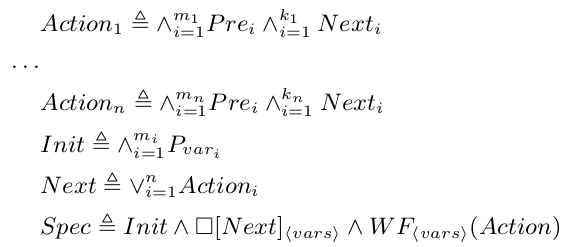
\includegraphics[width=6cm]{tla.png}
    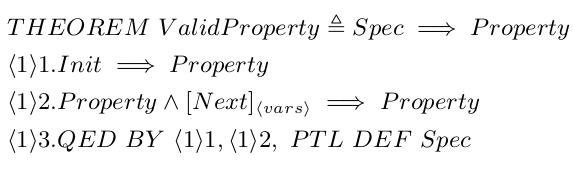
\includegraphics[width=6cm]{tlaps.png}
\end{figure}

$Action_{i}$ representa una acción, que se puede expresar como una conjunción de precondiciones y postcondiciones, donde la postcondición en general usa el valor de una variable en el próximo estado para describir la acción que se puede realizar dadas las precondiciones. \textit{Init} es el predicado de estado inicial, \textit{Next} es el predicado del siguiente estado válido, y \textit{Spec} es la especificación completa del sistema, que incluye el estado inicial, la relación de transición y condiciones de fairness, que puede ser débil o fuerte. Dada una acción A, la condición de fairness débil \textit{WF(A)} asegura que si A es habilitada permanentemente a partir de un estado, i.e. se cumplen las precondiciones de A, entonces A se ejecutará infinitas veces. La condición de fairness fuerte \textit{SF(A)} asegura que si A es habilitada frecuentemente a lo largo de una traza de estados, entonces A se ejecutará infinitas veces. El subíndice $\langle vars \rangle$ en \textit{Next} indican que puede darse que ninguna de esas variables cambien en un estado, y en las propiedades de fairness significa que el progreso debe darse para todas las variables del conjunto. 

Además, es posible con TLA+ formular teoremas y diseñar pruebas formales sobre propiedades de estas especificaciones en TLAPS. Un caso general puede enunciarse de la siguiente forma:

% \begin{footnotesize}
% \[
% \begin{aligned}
%     & THEOREM\ ValidProperty \triangleq Spec \implies Property \\
%     & \langle 1 \rangle1. Init \implies Property \\
%     & \langle 1 \rangle2. Property \land [Next]_{\langle vars \rangle} \implies Property \\
%     & \langle 1 \rangle3. QED\ BY\ \langle 1 \rangle1, \langle 1 \rangle2,\ PTL\ DEF\ Spec
% \end{aligned}
% \]
% \end{footnotesize}

donde definimos un teorema que permite probar Property a partir de la especificación, asistiendo la demostración con el contexto necesario para los motores de prueba, como la definición de Spec y propiedades básicas de lógica temporal proposicional.

Los modelos en TLA+ y su verificación en TLC ponen su foco en el comportamiento del sistema, abstrayéndose de los detalles de su implementación. Es por esto que son independientes de cualquier lenguaje de programación, y no es necesario anotar el programa. Sin embargo, es posible anotar el algoritmo usando el pseudo-código PlusCal, un lenguaje formal que se transpila a TLA+, para probar propiedades sobre sus variables. A diferencia del enfoque orientado a acciones, PlusCal se asemeja más a un lenguaje de programación imperativo y es más adecuado para especificar algoritmos secuenciales.

TLC visualiza los errores en las especificaciones de TLA+ proporcionando informes detallados cuando encuentra la violación de alguna propiedad. Cuando TLC detecta que una de las propiedades que está verificando no se cumple, procede a reportar un contraejemplo que ilustra cómo el sistema llega a un estado en el que esa propiedad es violada, a partir de un comportamiento válido segun la especificación. A continuación, TLC genera una traza que lleva al estado donde se produce la violación, representando cada estado como un predicado TLA+ que describe sus condiciones, y permite visualizar la evolución del sistema hasta llegar al estado problemático. Esta traza se minimiza para ofrecer una representación concisa pero informativa del problema. 

El verificador de modelos TLC permite la simulación de comportamientos del sistema. En modo de simulación, TLC construye y verifica repetidamente comportamientos individuales con una longitud máxima fija.

\section{Aspectos técnicos}
TLC representa el espacio de estado de manera explícita utilizando un grafo dirigido G cuyos nodos son los estados del sistema. Este grafo es una parte del grafo de alcanzabilidad del estado que TLC ha encontrado hasta el momento. Además, TLC mantiene una cola U de estados que aún no han sido visitados o cuyos sucesores aún no han sido calculados.

El model checker utiliza Breadth First Search para explorar los estados alcanzables de un sistema y verificar que cumplen con las invariantes especificadas. Comienza evaluando los supuestos y calculando los estados iniciales. A partir de estos estados, TLC los añade a una cola y un grafo si cumplen con las restricciones iniciales. Este método garantiza que todos los estados alcanzables se examinen sistemáticamente. Si TLC encuentra un estado sin sucesores posibles reporta un estado de deadlock, indicando que el sistema no puede progresar más desde ese punto.

TLC no considera todo el espacio de estado, sino una parte de él. Utiliza una técnica de exploración exhaustiva, pero debido a limitaciones de tiempo y de memoria, no es posible examinar todos los posibles estados de un sistema. En su lugar, TLC emplea estrategias inteligentes para explorar una porción representativa y significativa del espacio de estados, con el objetivo de detectar posibles problemas o violaciones de propiedades específicas en el modelo. Estas estrategias incluyen la generación de estados de manera incremental, el uso de técnicas de reducción como la simetría, y la exploración de estados que sean relevantes para las propiedades que se están verificando. De esta manera, TLC busca equilibrar la exhaustividad de la verificación con la eficiencia computacional, permitiendo obtener resultados significativos en un tiempo razonable.

En el contexto de TLA+, la simetría se aprovecha para reducir el número de estados que TLC necesita examinar al verificar una especificación. Si una especificación es simétrica con respecto a una permutación $\pi$, esto significa que si una secuencia de estados $\sigma$ satisface la especificación, entonces cualquier permutación de esa secuencia, $\sigma\pi$, también lo hará. Por lo tanto, si TLC ya ha verificado un comportamiento $\sigma$, no necesita verificar cualquier $\sigma\pi$ correspondiente, ya que cualquier error revelado por $\sigma$ también se revelaría por $\sigma\pi$.

En TLA+, se puede escribir una especificación de un programa que implementa una especificación más general mediante un mapeo de refinamiento adecuado. Este proceso implica mapear las variables de la especificación que se desea que el programa satisfaga con los estados de la especificación del programa en cuestión. El mapeo de refinamiento explica detalladamente cómo el programa cumple con la especificación general, lo que permite abstraer detalles específicos del programa y centrarse en su comportamiento general, asegurando que se cumplan las propiedades deseadas a nivel de especificación más alta.

En la verificación de modelos con TLC es posible que se generen falsos negativos, especialmente en el contexto de propiedades de liveness. Esto se debe a la dificultad de detectar violaciones de propiedades de liveness con modelos finitos, ya que estas propiedades requieren que el sistema alcance ciertos estados infinitas veces o en un orden específico, lo cual puede ser imposible de capturar con un modelo de estas características.

El procesamiento de TLAPS para probar un teorema, por su parte, es manejado por el TLAPM (TLA Proof Manager), que lee el archivo con la especificación en TLA+, y luego de ser analizado aplica una serie de transformaciones para enviarlo a motores de prueba externos, entre ellos SMT solvers (z3, cvc4, veriT), basados en método Tableaux (zenon), entre otros. 
Para probar una obligación de prueba el comportamiento por defecto es intentar resolverla con tres backends en secuencia, Z3, Zenon e Isabelle, con 5, 10, 30 segundos sus respectivos timeouts.
TLAPS ofrece muchas opciones para configurar timeouts, orden de solvers, y demás restricciones, el sistema de especificación es totalmente independiente. %% revisar referencias

\section{Casos de estudio}
\paragraph{Intel}
En Intel, TLA+ y TLC se han utilizado para diseñar y verificar protocolos de coherencia de caché en procesadores multinúcleo, en particular para los procesadores Alpha EV7 y EV8. En el caso de EV8 en particular, la especificación fue completada antes de que el diseño fuera estable, lo que brindó feedback temprano sobre la viabilidad del sistema a los diseñadores.

TLA+ facilita la exploración de optimizaciones y modificaciones del protocolo, permitiendo iteraciones rápidas y evaluaciones de su impacto en la complejidad del estado. La experiencia de los ingenieros de Intel mostró que TLA+ es una herramienta poderosa para encontrar errores y mejorar la eficiencia de los diseños complejos en etapas tempranas del desarrollo.

\paragraph{Amazon}
TLA+ se utiliza en Amazon Web Services (AWS) para corregir errores y mejorar la fiabilidad de diversos sistemas. El uso de herramientas de especificación formal y verificación de modelos permitió a los ingenieros verificar la corrección del sistema, comprender su funcionamiento interno y realizar optimizaciones de rendimiento sin sacrificar la corrección. La lista de proyectos donde Amazon utiliza esta herramienta incluye S3, DynamoDB, EBS (Elastic Block Store).

Debido al gran volumen de procesos que se realizan en los servidores de AWS, garantizar un código con la menor cantidad de bugs posible es esencial. Aunque un bug pueda parecer poco probable y tener una probabilidad de ocurrencia muy baja, la enorme cantidad de transacciones que se realizan diariamente hace que incluso estos casos poco probables puedan surgir. Es por esto que la capacidad de TLA+ para detectar y corregir incluso los errores más sutiles se vuelve crítica en un entorno donde la fiabilidad y la precisión son imperativas.

\paragraph{Prueba de un algoritmo tolerante a demoras y fallas de renombre de procesos}
En el marco de la computación paralela, se ha realizado un trabajo de análisis y verificación de un algoritmo no bloqueante y tolerante a fallas de renombre de procesos en un sistema de memoria compartido. Esto permite probar propiedades de safety y liveness sobre el sistema. En particular, se probó una propiedad que indica que cada proceso obtiene un nombre único, y otra que muestra que cada proceso que entra al sistema obtiene un nombre. Se realizaron, además, las pruebas pertinentes de corrección y completitud de los splitters, objetos que se utilizan para la sincronización de acciones sin bloqueo. Estas pruebas mostraban que los procesos son dirigidos en alguna dirección, derecha y abajo, con fairness en ambas, que solo se tiene un proceso asignado al nombre de ese splitter, y, finalmente, que cada proceso que entra al splitter es direccionado a alguna de estas categorias eventualmente.

\section{Caso de aplicación de la herramienta}
Se trata de un modelo de gestor de tareas, creado por el desarrollador Andreas Stührk. Este debe mantener actualizado el estado de realización de los trabajos encomendados, y asegurarse de que esto se gestione de manera concurrente. El sistema tenía un bug de consistencia en el supervisor de trabajos, y es que a veces no se percibía el cambio de ‘pendiente’ a ‘completo’. Entonces, desarrolló la especificación de las partes del sistema existente con TLA+, apoyándose también en el lenguaje de pseudocódigo asociado PlusCal, y chequeando invariantes de correctitud y progreso con TLC.

% \begin{wrapfigure}{r}{6cm}
%     \centering
%     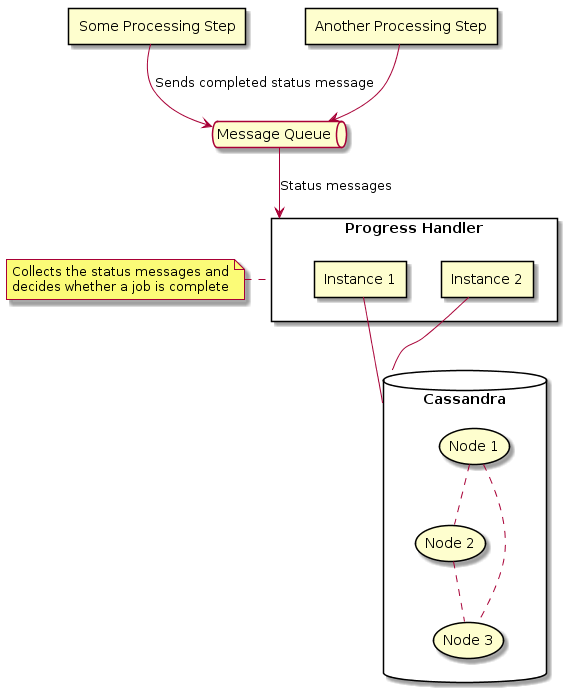
\includegraphics[width=4cm]{formalizing-the-system.png}
%     \caption{Arquitectura del sistema gestor de tareas.}
%     \label{caso_estudio}
% \end{wrapfigure}

Cada trabajo consiste en la completitud de tareas independientes. El sistema, a su vez, se compone de un supervisor de progreso, que toma los mensajes de estado de tareas de una cola FIFO conectada a las unidades de procesamiento, y decide si el trabajo está completo, almacenando la información del progreso en nodos en una unidad de almacenamiento (Cassandra). Esta unidad implementa factores de replicación y niveles de consistencia para asegurar que los datos sean replicados y leídos de manera confiable entre múltiples nodos. En Figura \ref{caso_estudio} se puede ver un diagrama de la arquitectura del sistema. 

En este trabajo se simplificó al máximo el modelo del sistema para atacar el problema de consistencia observado, modelando únicamente la operación de tomar un elemento de la cola.

Para el modelo de Cassandra se asume la implementación y correcto funcionamiento de la replicación automática de información en segundo plano. Luego, el modelo del nivel de consistencia consiste en escribir el mismo dato en los nodos especificados. La lectura de nodos se modela con la función $ReadProgress(nodes)$ como la unión de los progresos de $nodes$. A continuación se muestra el diseño del supervisor.

\begin{lstlisting}
\* Handles a progress message from the queue
fair process progressHandler \in {"handler1", "handler2"}
variable
    writeQuorumNodes \in NNodes(Quorum),
    readQuorumNodes \in NNodes(Quorum),
    secondReadQuorumNodes \in NNodes(Quorum),
    completedBefore = FALSE,
    message = "";
begin P0:
    while TRUE do
    Poll:
    recv(queue, message);
    unacked := unacked + 1;
    Read:
    completedBefore := ProcessingComplete(ReadProgress(readQuorumNodes));
    Write:
    call appendProgress(writeQuorumNodes, message);
    ReadAfterWrite:
    if ~completedBefore /\ ProcessingComplete(ReadProgress(secondReadQuorumNodes)) then
        \* The real progress handler would trigger some action here
        switchHappened := switchHappened + 1;
    end if;
    Ack:
    unacked := unacked - 1;
    end while;
end process;    
\end{lstlisting}

donde $unacked$ lleva la cuenta de mensajes procesandose por el supervisor, $switchHappened$ la cantidad de veces que se cambia el estado de ‘pendiente’ a ‘completo’ de un trabajo, y $queue$ la cola de mensajes con tareas completas por las unidades de procesamiento.

Podemos entonces definir las propiedades a verificar en el modelo. En primer lugar, el invariante de correctitud, que asegure que o bien quedan tareas aún no procesadas como completas (cola no vacía), o bien el manejador está procesando un mensaje de status (\(unacked > 0\)), o bien ya se ha completado el trabajo y se puede visualizar en el supervisor (\(switchHappened > 0\)). Definimos además, la propiedad de progreso esperada, que denote que el supervisor cambia de estado eventualmente.

\begin{wrapfigure}[6]{l}{6.5cm}
\begin{lstlisting}
Correctness == \/ queue # <<>>
                 \/ unacked > 0
                 \/ switchHappened > 0    

Liveness == <>[](switchHappened > 0)
\end{lstlisting}
\end{wrapfigure}

Esta especificación logró poner en evidencia el error. En el diseño del sistema se puede demostrar que es necesario hacer lecturas y escrituras por quórum en los nodos de Cassandra, indicando que la lectura de un único nodo no es confiable, ya que este puede no haber sido actualizado por algún interleaving con otra lectura del proceso. Al analizar más profundamente, se descubrió que en la implementación real las lecturas de la base de datos no usaban niveles de consistencia de quórum correctamente.

El código usa Java con la librería Datastax Cassandra Driver statements con el siguiente formato:
% \begin{wrapfigure}{l}{8.5cm}
\begin{lstlisting}[language=Java]
Statement insert = QueryBuilder
.insertInto(keyspace, columnFamily)
// Omitted: binding expressions for the values here
.setConsistencyLevel(consistencyLevel);
return session.prepare(insert.toString());
\end{lstlisting}
% \end{wrapfigure}

El bug se encuentra en esta sección, ya que no se incluye la propiedad del nivel de consistencia en la representación en string de la consulta, por lo que el siguiente cambio enmienda el error:
%
\begin{lstlisting}
Statement insert = QueryBuilder
.insertInto(keyspace, columnFamily)
// Omitted: binding expressions for the values here
return session
.prepare(insert.toString());
.setConsistencyLevel(consistencyLevel);
\end{lstlisting}

%
Por otra parte, es posible ver una limitación en el diseño, ya que no puede probarse la propiedad que especifica que el cambio de estado de ‘pendiente’ a ‘completo’ se observa a lo sumo una vez ( \([NoDupSwitch == switchHappened <= 1]\) ), implicando el riesgo de reportar como completado más de una vez un trabajo.

\section{Conclusiones}

TLA+ es accesible para aquellos con conocimientos básicos en lógica y teoría de conjuntos. Tiene una sintaxis que simula la matemática clásica, y el model checker tiene un funcionamiento muy similar a otros del mismo nivel de expresividad.

TLAPS puede resultar más complejo de manjear que TLA+, ya que hay que definir el contexto adecuado de prueba de un teorema, lo cual puede requerir de un esfuerzo considerable, sobre todo si no se tiene una idea de la validez del diseño desde el principio. 

La instalación de TLA+ y sus herramientas asociadas es generalmente sencilla y bien documentada.

Las herramientas de TLA+ pueden ser muy útiles para la corrección de diseño (tendo dudas acá). Según la experiencia de expertos, estas herramientas han sido efectivas en la identificación de bugs que podrían haber pasado desapercibidos con métodos de testing convencionales.

TLA+ puede verificar programas de diversos tipos, demostrando su versatilidad y adaptabilidad a diferentes contextos y necesidades en el desarrollo de sistemas.

En general, TLA+ y TLAPS son herramientas poderosas que, a pesar de su potencial complejidad inicial en ciertos aspectos, se presentan como una herramientas altamente recomendables para aquellos involucrados en el diseño y verificación de sistemas, debido a su capacidad para mejorar la calidad y fiabilidad de los sistemas desarrollados. 

\begin{thebibliography}{8}
\bibitem{wiki}
Wikipedia, La Enciclopedia Libre, "TLA+", \url{https://en.wikipedia.org/wiki/TLA%2B}, último acceso 2024/05/28

\bibitem{tlaps}
TLA+ Proof System, \url{https://proofs.tlapl.us/doc/web/content/Home.html}, último acceso 2024/05/28

\bibitem{tla}
The TLA+ Home Page, \url{https://lamport.azurewebsites.net/tla/tla.html}, último acceso 2024/05/28

\bibitem{tla_history}
TLA+ in Practice and Theory. Part 1: The Principles of TLA+, \url{https://pron.github.io/posts/tlaplus_part1}, último acceso 2024/05/30

\bibitem{case_study}
Finding bugs in systems through formalization, \url{https://andy.hammerhartes.de/finding-bugs-in-systems-through-formalization.html}, último acceso 2024/05/28

\bibitem{amazon}
Chris N., Tim R., Fan Z., Bogdan M., Marc B., Michael D.: Use of Formal Methods at Amazon Web Services. Amazon.com, 29th September, 2014

\bibitem{elastic_search}
Possible to index duplicate documents with same id and routing id, \url{https://github.com/elastic/elasticsearch/issues/31976#issuecomment-404722753}

\bibitem{book}
Leslie L.: Specifying Systems: The TLA+ Language and Tools for Hardware and Software Engineers. Addison-Wesley Professional, 2002

\end{thebibliography}
\end{document}
